\documentclass[12pt]{cspcccsthesis}
% preamble

\title{COMPARATIVE ANALYSIS OF DISCRETE-EVENT AND CONTINUOUS SIMULATION MODELS FOR STUDENTS FLOW OPTIMIZATION}
\authorOne{Author Name 1}
\authorTwo{Author Name 2}
\authorThree{Author Name 3}
\authorFour{Author Name 4}
\authorFive{}
\degree{Bachelor of Science in Computer Science}
\approvaldate{January 1, 2020}
\school{College of Computer Studies}
\adviser{Adviser Name}
\dean{Challiz D. Omorog, DIT}
\committeeMemberOne{Dr. John Smith}
\committeeMemberTwo{Dr. Jane Doe}
\committeeChair{Dr. Alex Johnson}
\department{}
\thesisAbstract{Lorem ipsum dolor sit amet, consectetur adipiscing elit. Nunc scelerisque hendrerit fringilla. Vestibulum nec nibh nisi. Curabitur iaculis est lorem, vehicula consectetur erat ullamcorper eget. Aliquam cursus mollis pretium. Fusce bibendum ornare nisl quis dictum. Curabitur tincidunt euismod erat, fringilla elementum ex blandit in. Nunc pretium libero non bibendum egestas. Interdum et malesuada fames ac ante ipsum primis in faucibus. Etiam vitae porttitor eros. Suspendisse pretium feugiat dui, sed posuere erat porta eu. Lorem ipsum dolor sit amet, consectetur adipiscing elit. Nunc scelerisque hendrerit fringilla. Vestibulum nec nibh nisi. Curabitur iaculis est lorem, vehicula consectetur erat ullamcorper eget. Aliquam cursus mollis pretium. Fusce bibendum ornare nisl quis dictum. Curabitur tincidunt euismod erat, fringilla elementum ex blandit in. Nunc pretium libero non bibendum egestas. Interdum et malesuada fames ac ante ipsum primis in faucibus. Etiam vitae porttitor eros. Suspendisse pretium feugiat dui, sed posuere erat porta eu}
\keywords{amet, consectetur, adipisci velit}

% Load glossary entries
\newacronym{starlabs}{S.T.A.R. Labs}{Scientific and Technological Advanced Research Laboratories}

% Add other glossary entries below as needed 

% document body
\begin{document}

\makeTitlePage{January}{2022}

\begin{frontmatter}
    % In \begin{approvalPage}{N}, the parameter N is the number of members in the committee. If this is less than 4, the layout of the page is single-column rather than two-column, so change the value accordingly.

\begin{approvalPage}{3}
    
% Add people in the following format:
% \committeeMember{Member Name}{Member Department/Position}{Member Affiliation}

\end{approvalPage}

    \makePanelofExaminers{90}
    \makeDedication{Ad Majorem Dei Gloriam}
    
\begin{acknowledgments}

I would like to thank the members of my thesis committee for their help in preparation of this work -- Niles Caulder, without whom I would have been doomed to never complete it, Kimiyo Hoshi, who helped to shed new light on many of my ideas, Pamela Isley, with whom I often disagree but who inspires me to be better, Raymond Palmer, who had no small part to play in the formation of the idea, and Kent Nelson, who always had golden advice.

Special thanks are due to the friends and colleagues who made this work possible. Jimmy Olsen and Pete Ross were invaluable both as friends and as sounding boards for some of my more outlandish ideas. Jack Knight, who I met only briefly, was a major influence, and I'm glad we were able to help each other. 

The author gratefully acknowledges the support for this work offered by S.T.A.R. Laboratories under grant award number 3X29YZ4A, and by the Theodore S. Kord Fellowship. Any views and conclusions contained herein are those of the author, and do not necessarily represent the official positions, express or implied, of the funders.

\end{acknowledgments}

    \makeAbstract
    \makeTOC
    \makeListOfTables
    \makeListOfFigures
\end{frontmatter}

\begin{thesisbody}
    \chapter{Introduction}
\begin{refsection}
\section{Background of the Problem}

It is common knowledge that the star closest to Earth is the Sun, and also that the Sun is yellow. It is this yellow sunlight which is interesting for some of its properties \cite{onate_exploring_2021} \cite{scholes2011lessons}. For instance, plants, algae, and cyanobacteria convert this light into energy via photosynthesis. In \ref{fig:firstFig} is a photo of a galaxy which contains many stars.


\begin{equation}
	x = \frac{-b \pm \sqrt{b^2 - 4ac}}{2a}
\end{equation}


\begin{figure}[ht]
    \centering
	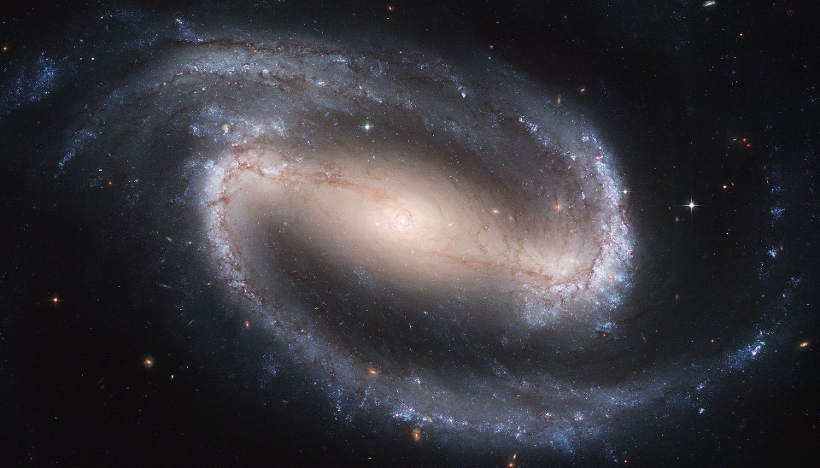
\includegraphics[width=0.85\textwidth]{figures/sampleFig1.jpg} 
	\caption[Barred spiral galaxy NGC 1300]{Barred spiral galaxy NGC 1300}
	\label{fig:firstFig}
\end{figure}

\ref{fig:firstFig}

The stars in the sky are of particular interest to the aptly named S.T.A.R. Labs, which in many recent experiments has shown promising results in converting this energy in a non-photoelectric sense into usable energy \cite{ssdsdsd_solid_2012}. Interestingly, \gls{starlabs} has theorized that the famous superhero known as ``Superman'' converts the light from our sun, which grants his fantastic abilities. There are many methods in industry for converting the sun's energy (of about \SI{1000}{\watt\per\meter\squared}) into electrical energy. Some of these are highlighted in \ref{tbl:sampleTbl1} \cite{noauthor_techopedia_nodate}.

\begin{table}[ht]
\centering
\caption{This is a table}
\label{tbl:sampleTbl1}
\resizebox{0.8\textwidth}{!}{%
\begin{tabular}{llll}
\hline
installation & type & capacity (GW) & location \\ \hline
Longyangxia Dam & photovoltaic & 0.85 & China \\
Gansu Wind Farm & wind & 6 & China \\
Sihwa Lake & tidal & 0.254 & South Korea \\ \hline
\end{tabular}%
}
\end{table}

\section{Statement of the Problem}

Enter the statement of the problem here. To cite a study add a bib entry in the references.bib, then use this code \cite{noauthor_biblatex_nodate} to cite the study.

\section{Objectives of the Study}

\subsection{General Objective}

Enter your General Objective here.

\subsection{Specific Objectives}

More Specifically, this study aims to:

\begin{enumerate}
    \item To write this research paper
    \item To present it in the title defense.
\end{enumerate}
   

\section{Significance of the Study}

Write your Significance of the study here.

\section{Scope and Limitation}

State the scope and limitation of your study here.

\section{Project Dictionary}

The Project Dictionary contains the technical terms that defined the conceptual and operation of this study:

\begin{itemize}
    \item \textbf{Convolutional Neural Network (CNN, or ConvNet).} is a class of artificial neural network, most commonly applied to analyze visual imagery. They are also known as shift invariant or space invariant artificial neural networks (SIANN), based on the shared-weight architecture of the convolution kernels or filters that slide along input features and provide translation equivariant responses known as feature maps.
    \item \textbf{Digital image processing} is the use of a digital computer to process digital images through an algorithmis the use of a digital computer to process digital images through an algorithmis the use of a digital computer to process digital images through an algorithmis the use of a digital computer to process digital imais the use of a digital computer to process digital images through an algorithmis the use of a digital computer to process digital images through an algorithmis the use of a digital computer to process digital images through an algorithmges through an is the use of a digital computer to process digital images is the use of a digital computer to process digital images through an algorithmis the use of a digital computer to process digital images through an algorithmis the use of a digital computer to process digital images through an algorithmthrough an algorithmis the use of a digital computer to process digital images through an algorithmalgorithmis the use of a digital computer to process digital images through an algorithm \cite{scholes2011lessons}. 
\end{itemize}

% Then replace \subfloat with \begin{subfigure} in your code:
	
\begin{figure}[H]
	\centering
	
	% Row 1
	\begin{subfigure}[b]{0.40\textwidth}
		\centering
		\fbox{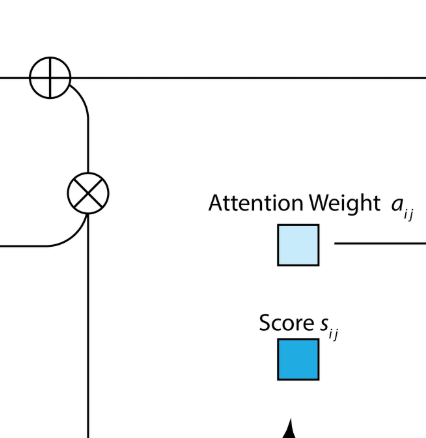
\includegraphics[width=1\textwidth]{figures/imageA.png}}
		\caption{Caption for subfigure a}
		\label{fig:firstFig:a}
	\end{subfigure}
	\hfill
	\begin{subfigure}[b]{0.40\textwidth}
		\centering
		\fbox{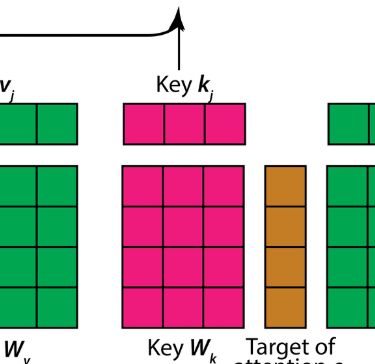
\includegraphics[width=1\textwidth]{figures/imageB.png}}
		\caption{Caption for subfigure b}
		\label{fig:firstFig:b}
	\end{subfigure}
	
	\vspace{1em}
	
	% Row 2
	\begin{subfigure}[b]{0.40\textwidth}
		\centering
		\fbox{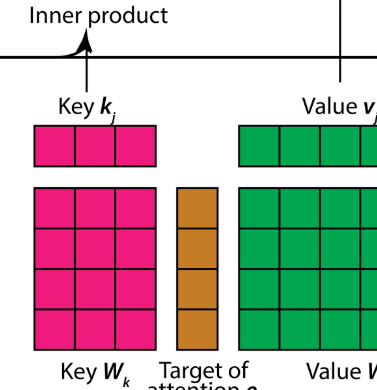
\includegraphics[width=1\textwidth]{figures/imageC.png}}
		\caption{Caption for subfigure c}
		\label{fig:firstFig:c}
	\end{subfigure}
	\hfill
	\begin{subfigure}[b]{0.40\textwidth}
		\centering
		\fbox{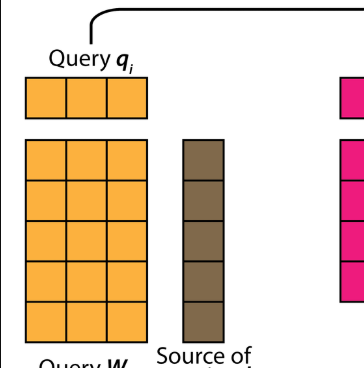
\includegraphics[width=1\textwidth]{figures/imageD.png}}
		\caption{Caption for subfigure d}
		\label{fig:firstFig:d}
	\end{subfigure}
	
	\caption{Main caption for the entire figure showcasing four different aspects.}
	\label{fig:subsubfigwithlabel}
\end{figure}


This is sample in-text citation of \ref{fig:subsubfigwithlabel} and \ref{fig:firstFig:d}.



%=======================================================%
%%%%% Do not delete this part %%%%%%
\clearpage

\printbibliography[heading=subbibintoc, title={\texorpdfstring{\centering}{} Notes}]
\end{refsection}
    
\chapter{Related Literature and Studies}
\begin{refsection}

The process of data collection began with analysis of the physical principles underlying optical light emission. For illustration purposes, see \ref{fig:secondFig}.

\section{Review of Related Literature and Studies}


Depending on the energy of a photon, it may be referred to as ``light'' (in the case of optical photons) or as something else -- for example, a gamma ray. By convention, there are many names for these particles \citeauthor{allen2019fast} [\citeyear{allen2019fast}].

\subsection{Low-energy photons}

The lowest energy electromagnetic radiation is carried by radio waves.

\subsection{Intermediate-energy photons}

These include several types of radiation, including the usually-harmful.

\subsubsection{Microwaves}

Microwaves have wavelengths on the order of \SI{1e-2}{\meter}, or a few \si{\centi\meter}.

\subsubsection{Visible light}

Visible light is that which is detectable by the human eye, with wavelengths about \SIrange{380}{750}{\nano\meter}.

\begin{rotatepage}
\begin{sidewaysfigure}[!t]
    \centering
    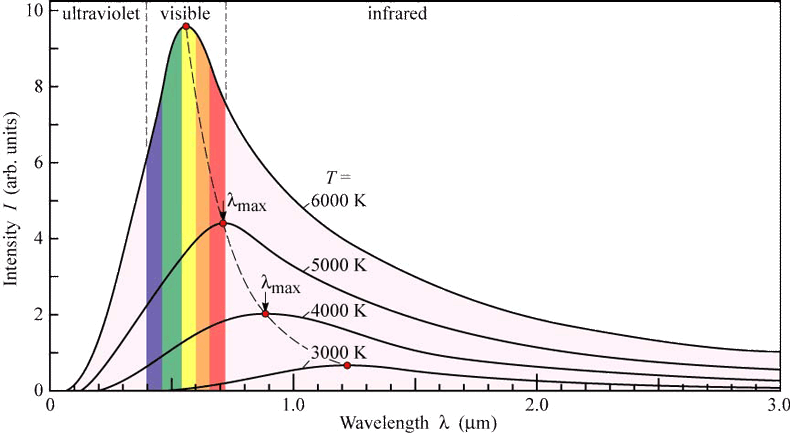
\includegraphics[width=\textwidth]{figures/sampleFig2.png}
    \caption[Black-body radiation ddd dddd dddd]{Spectra of black-body radiation at various temperatures, according to Wien's displacement law \cite{wannier1987statistical}.}
    \label{fig:secondFig}
\end{sidewaysfigure}
\end{rotatepage}

\begin{figure}[ht]
    \centering
	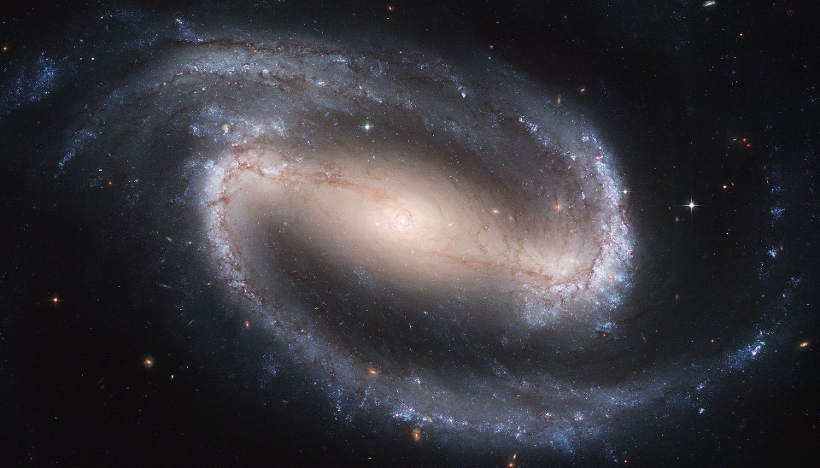
\includegraphics[width=0.85\textwidth]{figures/sampleFig1.jpg} 
	\caption[Barred spiral galaxy NGC 1300]{Barred spiral galaxy NGC 1300 photographed by Hubble telescope. While the galaxy in the photo is not our sun, it does emit light, much like our sun. Image credit: NASA.}
	\label{fig:firstFig}
\end{figure}



%=======================================================%
%%%%% Do not delete this part %%%%%%
\clearpage

\printbibliography[heading=subbibintoc, title={\texorpdfstring{\centering}{} Notes}]
\end{refsection}
    
\chapter{Methodology}
\begin{refsection}
% text of this chapter goes here

\begin{figure}[ht]
    \centering
	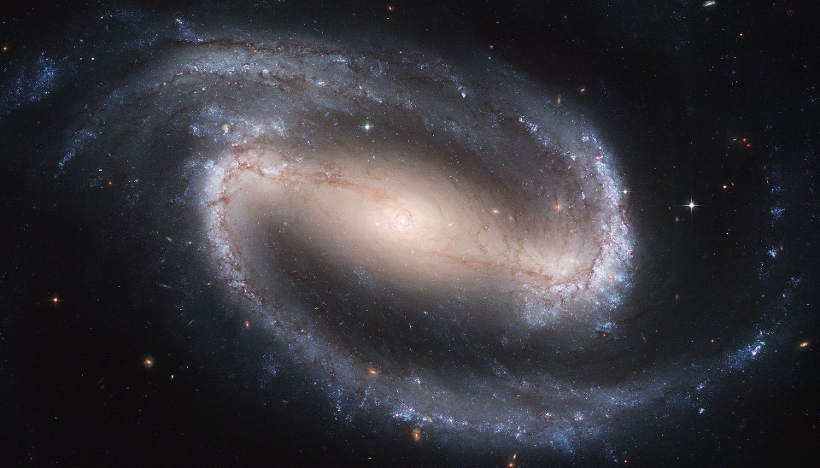
\includegraphics[width=0.85\textwidth]{figures/sampleFig1.jpg} 
	\caption[Barred spiral galaxy NGC 1300]{Barred spiral galaxy NGC 1300 photographed by Hubble telescope. While the galaxy in the photo is not our sun, it does emit light, much like our sun. Image credit: NASA.}
	\label{fig:firstFig}
\end{figure}

%=======================================================%
%%%%% Do not delete this part %%%%%%
\clearpage

\printbibliography[heading=subbibintoc, title={\texorpdfstring{\centering}{} Notes}]
\end{refsection}
    
\chapter{Results and Discussion}
\begin{refsection}

\begin{figure}[ht]
    \centering
	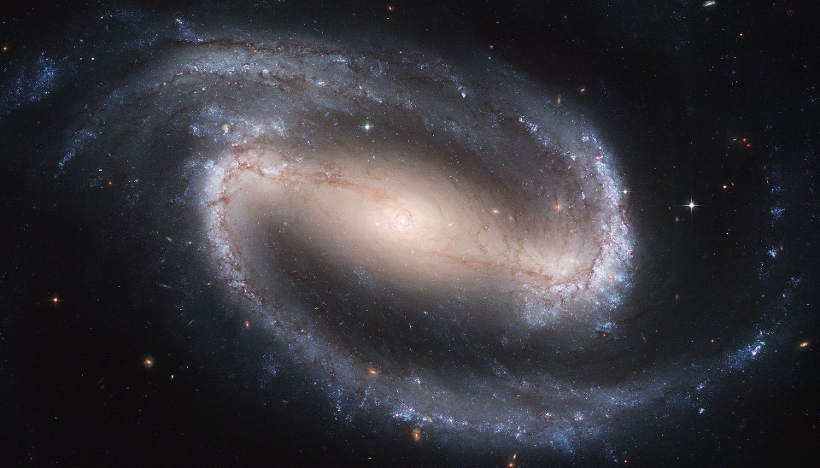
\includegraphics[width=0.85\textwidth]{figures/sampleFig1.jpg}
	\caption[Barred spiral galaxy NGC 1300]{Barred spiral galaxy NGC 1300 photographed by Hubble telescope. While the galaxy in the photo is not our sun, it does emit light, much like our sun. Image credit: NASA.}
	\label{fig:firstddd}
\end{figure}






%=======================================================%
%%%%% Do not delete this part %%%%%%
\clearpage

\printbibliography[heading=subbibintoc, title={\texorpdfstring{\centering}{} Notes}]
\end{refsection}
    
\chapter{Conclusion}
\begin{refsection}
% text of this chapter goes here


\begin{figure}[ht]
    \centering
	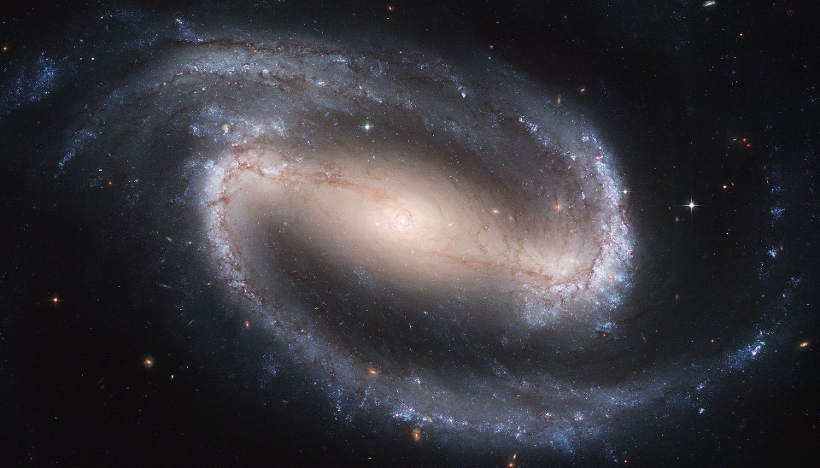
\includegraphics[width=0.85\textwidth]{figures/sampleFig1.jpg} 
	\caption[Barred spiral galaxy NGC 1300]{Barred spiral galaxy NGC 1300 photographed by Hubble telescope. While the galaxy in the photo is not our sun, it does emit light, much like our sun. Image credit: NASA.}
	\label{fig:firstFig}
\end{figure}


%=======================================================%
%%%%% Do not delete this part %%%%%%
\clearpage

\printbibliography[heading=subbibintoc, title={\texorpdfstring{\centering}{} Notes}]
\end{refsection}
    \makeBibliography
    
% The environment used here (theappendices) is a wrapper for the basic appendices environment which changes the appearance of the title page and the structure and appearance of the appendices in the table of contents and PDF bookmarks. The original functionality can be restored by simply removing the 'the' from the \begin{} and \end{} statements below.

\begin{theappendices}

\chapter{Language Editing Certification}
\centering

This is to certify that the undersigned has reviewed and went through all the pages of the Bachelor of Science in Computer Science thesis manuscript titled \\

\textbf{"ENTER YOUR TITLE HERE"} \\


of \textbf{AuthorName1}, \textbf{AuthorName2}, \textbf{AuthorName3}, as against the set of structural rules that govern research writing in accord with the composition of sentences, phrases, and words in the English language.
 \newline \newline \newline \\

\noindent \textbf{JUAN DE LA CRUZ} \\
\textit{Language Editor} \\

Date:\_\_\_\_\_\_\_\_\_\_\_\_\_\_\_\_\_\_\_\_\_\_\_


\chapter{Secretary's Certification}
\centering

This is to certify that the undersigned has provided accurate recommendations, suggestions, and comments unanimously agreed and approved by the panel of examiners during the oral examination of the thesis titled \\ \textbf{"ENTER YOUR TITLE HERE"} \\  prepared and submitted by \textbf{AuthorName1}, \textbf{AuthorName2}, \textbf{AuthorName3}, and that the same have not been amended, modified or obliterated. \newline \newline \newline \\



\textbf{MS. MARIA DAISY R. BELARDO} \\
\textit{Secretary} \\


Date:\_\_\_\_\_\_\_\_\_\_\_\_\_\_\_\_\_\_\_\_\_\_\_

\chapter{JOINT AFFIDAVIT OF UNDERTAKING (Plagiarism)}

\centering

\textbf{JOINT AFFIDAVIT OF UNDERTAKING}


% IN WITNESS WHEREOF, I have hereunto set my name this ____ day of ___________ 202__ in
% ___________________________________, Philippines.
% SUBSCRIBED AND SWORN TO before me this ___ day of ________ at _______________, Philippines,
% affiants exhibiting to me their competent proofs of identity above stated.
% Doc. No. ___________:
% Page No.: __________:
% Book No.: __________:
% Series of 202_.


\end{theappendices}
    % Vita should only be included for PhD candidates.

\begin{vita}

\begin{itemize}
    \item 
    
    \begin{figure}[ht]
        \centering
    	
\includegraphics[width=0.35\textwidth]{figures/person-icon.png}
    \end{figure}
    
    \textbf{Joseph Jessie S. Oñate} is a faculty member of the College of Computer Studies. He finished his Master of Science in Computer Science degree at Ateneo de Naga University. His research interests focused on Intelligent Systems, Algorithm and Complexity, Web Technologies, Computer Vision, and Graphics.
    
    \item 
    
    \begin{figure}[ht]
        \centering
    	
\includegraphics[width=0.35\textwidth]{figures/person-icon.png}
    \end{figure}
    
    \textbf{Joseph Jessie S. Oñate} is a faculty member of the College of Computer Studies. He finished his Master of Science in Computer Science degree at Ateneo de Naga University. His research interests focused on Intelligent Systems, Algorithm and Complexity, Web Technologies, Computer Vision, and Graphics.
    
    \item 
    
    \begin{figure}[ht]
        \centering
    	
\includegraphics[width=0.35\textwidth]{figures/person-icon.png}
    \end{figure}
    
    \textbf{Joseph Jessie S. Oñate} is a faculty member of the College of Computer Studies. He finished his Master of Science in Computer Science degree at Ateneo de Naga University. His research interests focused on Intelligent Systems, Algorithm and Complexity, Web Technologies, Computer Vision, and Graphics.
\end{itemize}

\end{vita}
\end{thesisbody}

\end{document}
